\section{Testsubject QA Makefile}
\label{example:testsubjectQA}

This is an example of using a makefile to create quality assurance (QA) images, and then generate a final QA report in HTML using R Markdown. 

The code for this example is in \texttt{testsubject/lib/makefiles/QA.mk}, and it is included by\linebreak \texttt{testsubject/test001/Makefile}.

\setcounter{codehighlight}{0} % RESET THIS BEFORE EVERY LST LISTING
\begin{lstlisting}
	%*\lnote*NIPYPATH=/usr/local/anaconda/bin
	FSL_DIR=/usr/share/fsl/5.0

	%*\lnote*.PHONY: TNSR MotionGraphs SkullstripQA QAReport

	%*\lnote*qa:   $(call print-help, qa, Create QA report) TSNR MotionGraphs SkullstripQA QAreport
\end{lstlisting}

\noindent\lnum{1} As is customary in a makefile, we first define paths
to locations that we want to refer to later on. \\
\lnum{2} Here, our phony targets are targets that are not actual files.\\
\lnum{3} This line tells the \maken{} help system what to do when you
are unsure of what this makefile does. Here, it will print out what
the \texttt{qa} target does (i.e., create a QA report). See \nameref{sec:practicum4} for more information about the help system. \\

\begin{lstlisting}
	%*\lnote*TSNR: QA/images/rest_tsdiffana.gif

	QA/images/%_tsdiffana.gif: rest.nii.gz
		%*\lnote*mkdir -p QA/images ;\
		%*\lnote*pngout= %*\`{}*echo $@|sed `s/gif/png/g'%*\`{}* ;\
		%*\lnote*$(NIPYPATH)/nipy_tsdiffana --out-file $$pngout $< ;\
		convert $$pngout $@ ;\
		rm -f $$pngout
\end{lstlisting}

\noindent\lnum{4} Our first target creates TSNR images for the QA. In this example, the phony target TSNR only wants \maken{} to create a single \texttt{gif} image. \\
\lnum{5} This line creates a directory called \texttt{QA/images} if it does not already exist. The \texttt{-p} flag tells \texttt{mkdir} not to throw an error if that directory exists, but create it if it does not.
\lnum{6} The variable \texttt{pngout} is defined to take the filename of your target and substitute \texttt{gif} with \texttt{png}.\\
\lnum{7} Subsequently, the code calls the script \texttt{nipy\_tsdiffana} which is located in the directory \texttt{\$(NIPYPATH)} you defined earlier.\\ The python script will generate a \texttt{png} image comprised of 4 graphs showing the scaled variance, slice-by-slice variance, scaled mean voxel intensity and the max/mean/min slice variation of your resting-state time series, as seen in the image below. \\

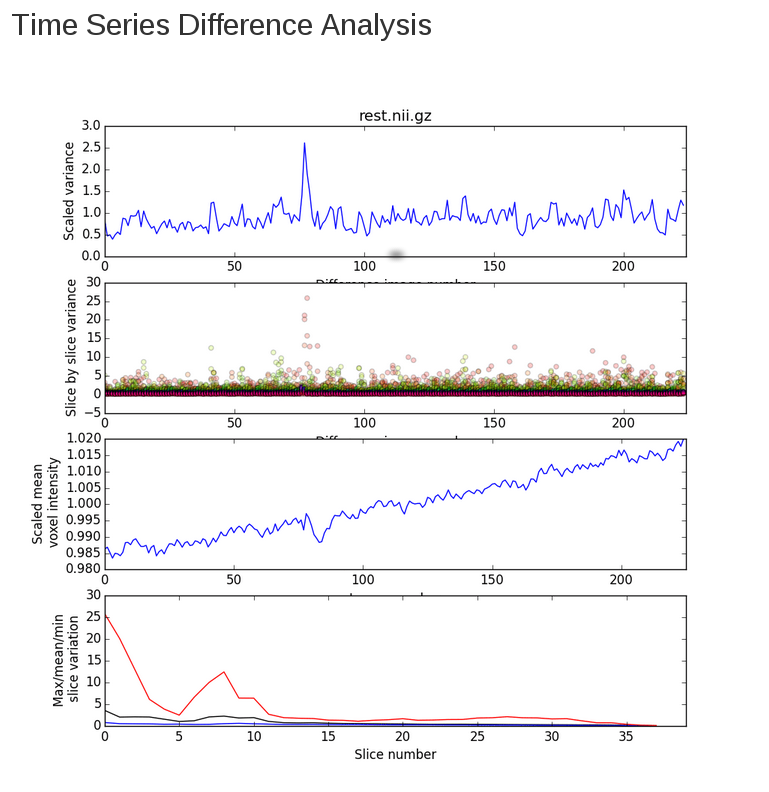
\includegraphics[scale=0.5]{images/QAtsdiffana.png}

\begin{lstlisting}
	MotionGraphs: QA/images/rest_MotionGraphRotations.gif 

	QA/images/rest_MotionGraphRotations.gif: rest_dir/rest_mc.nii.gz
		%*\lnote*$(PROJECT_HOME)/bin/R/MakingGraphs.Rscript  QA/images rest
\end{lstlisting}

\lnum{8}  \texttt{MakingGraphs.Rscript} is a R script that will generate 4 separate graphs for you: \\
	\tab 1. A motion rotations graph showing rotations along the x/y/z planes.\\
	\tab 2. A motion translations graph showing translations along the x/y/z planes.\\
	\tab 3. A framewise displacement (FD) graph to show displacement in mm across acquired volumes.\\
	\tab 4. A signal intensity (DVARS) graph to show signal intensity across acquired volumes.\\
	To understand the usage of an R script, it is usually necessary to look at the code itself. In this line, the R script called with the output directory \texttt{QA/images} as the first argument, followed by the prefix \texttt{rest} to be used for naming the output images.\\

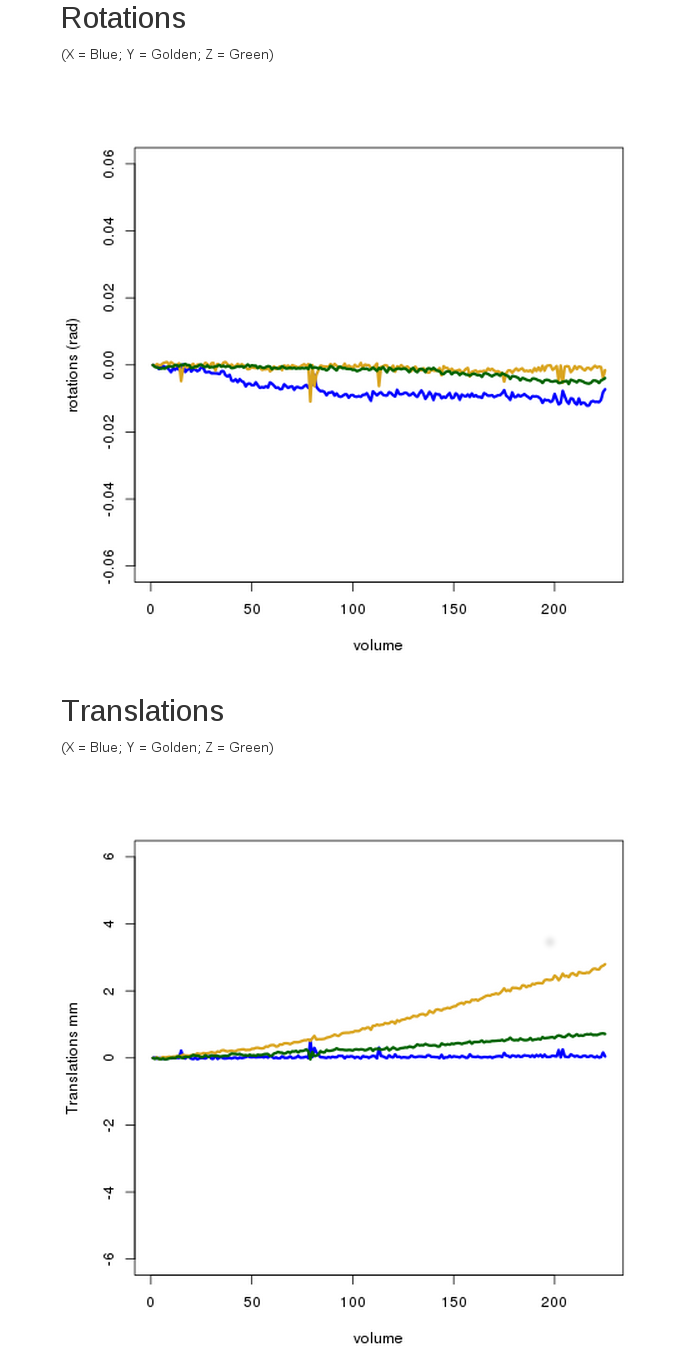
\includegraphics[scale=0.3]{images/QAmotion1.png}
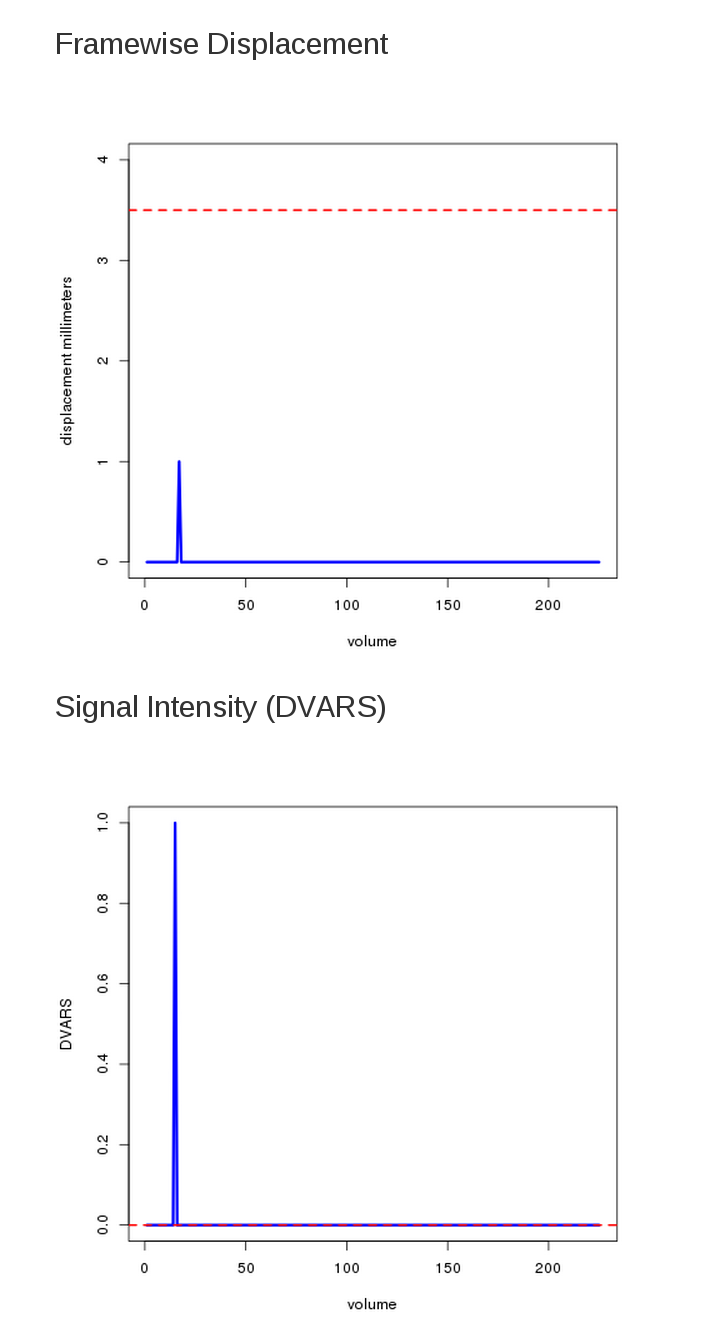
\includegraphics[scale=0.3]{images/QAmotion2.png}

\begin{lstlisting}
	SkullstripQA: QA/images/T1_skstrip.gif

	QA/images/T1_skstrip.gif: T1.nii.gz T1_skstrip_mask.nii.gz
		mkdir -p QA/images ;\
		%*\lnote*$(FSL_DIR)/bin/overlay 1 1 $< -a $(word 2,$^) 1 10 \
		rendered_T1_brain.nii.gz ;\
		%*\lnote*$(PROJECT_HOME)/bin/slices rendered_T1_brain.nii.gz \
		-o %*\`{}*dirname $@%*\`{}*/%*\`{}*basename $@ .gif%*\`{}*.png ;\
		%*\lnote*convert %*\`{}*dirname $@%*\`{}*/%*\`{}*basename $@ .gif%*\`{}*.png -resize 500 $@ ;\
		rm rendered_T1_brain.nii.gz ;\
		rm %*\`{}*dirname $@%*\`{}*/%*\`{}*basename $@ .gif%*\`{}*.png

\end{lstlisting}


To ensure that our skull-strip does not remove too much of the brain or too little of the skull, we can create an image to overlay the skull-stripped mask generated from \texttt{resting.mk} on top of the T1 brain. \\
\tab\lnum{9} FSL \texttt{overlay} is a tool that is used to overlay a 3D images over another. It is capable of overlaying a maximum of 2 images on top of a reference image. Type \texttt{overlay} into your command line to understand how it is used. In this line, we call \texttt{overlay}. The \texttt{1}s that are provided as arguments specify the color and output type of your overlay. The next argument is the background image, which in this case is the first dependency we have listed, i.e. \texttt{T1.nii.gz}. The \$\textasciicircum{} refers to this file. The final output image is called \texttt{rendered\_T1\_brain.nii.gz}. Again, to understand the flags, you must look at overlay's usage. \\
\lnum{10} FSL \texttt{slices} is a script that calls the FSL tool \texttt{slicer} to create an image consisting of 3 axial, 3 sagittal and 3 coronal slices. Here, we feed it the \texttt{rendered\_T1\_brain.nii.gz} file that we want FSL \texttt{slices} to use. The output will be a file called \texttt{QA/images/T1\_skstrip.png}. Instead of typing out the full name of the file, however, we simply provide the directory name and basename of our target and replace \texttt{.gif} with \texttt{.png}. \\
\lnum{11} Following this, we convert our PNG image into a GIF image, using ImageMagick's \texttt{convert} that performs the conversion and resizes the image.\footnote{This step was necessary in earlier versions of R Markdown that had trouble including PNG images, but may not be necessary for you.}\\

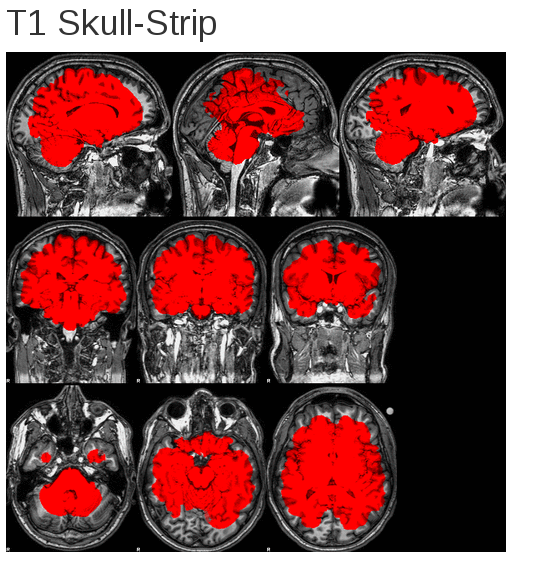
\includegraphics[scale=0.4]{images/QAskullstrip.png}

\begin{lstlisting}
	QAreport: QA/rest_Preprocessing.html 

	QA/rest_Preprocessing.html: $(PROJECT_HOME)/lib/Rmd/fMRI.Rmd TSNR MotionGraphs SkullstripQA
		%*\lnote*sed -e `s/SUBJECT/$(subject)/g' -e `s/TASK/rest/g' $(word 1,$^) > \
		QA/rest_Preprocessing.Rmd ;\
		%*\lnote*R -e `library("rmarkdown"); \
		rmarkdown::render("QA/rest_Preprocessing.Rmd")' ;\
		rm -f QA/rest_Preprocessing.Rmd QA/rest_Preprocessing.md
\end{lstlisting}


Finally, to generate our QA HTML report, we use R Markdown. We do this by writing a file called \texttt{fMRI.Rmd}, which is the first dependency listed here. The \texttt{fMRI.Rmd} file reads the QA images that were generated in the previous portions of this makefile to create a HTML page (see \nameref{sec:practicum4} for a brief explanation of what goes into a Rmd file and how to write one). \\
\lnum{12} In this line, we substitute pattern strings in the \texttt{fMRI.Rmd} file with variables that have been defined in the makefiles by using \texttt{sed}. \texttt{SUBJECT}, for instance, will be replaced with the \texttt{\$(subject)} variable defined in the main makefile \texttt{\$(PROJECT\_HOME)/test001/Makefile}. \texttt{TASK} will be replaced with \texttt{rest}, because we are only interested in looking at the QA report for resting-state functional scans for now. We can define another variable called \texttt{task} if we have several types of runs that we want to generate QA reports for (e.g., task runs or multiple resting state runs). Once the pattern strings have been substituted, the \texttt{fMRI.Rmd} file will be copied over to the \texttt{QA} directory and be renamed as \texttt{rest\_Preprocessing.Rmd}. \\
\lnum{13} This line tells R to load the `\texttt{rmarkdown}' library so that it can read the R Markdown file. R will then render \texttt{QA/rest\_Preprocessing.Rmd} to create your HTML report! \\

To view the full report, you can open the file \texttt{testsubject/test001/QA/rest_Preprocessing_example.html} in a browser.


\begin{lstlisting}
		clean_qa: 
		rm -rf QA
\end{lstlisting}

Finally, with other makefiles, we define a \texttt{clean} target specifically for QA. Because quality assurance is an intermediate step in the neuroimaging processing pipeline, we do not necessarily need to retain the QA images and reports once they have been checked.


